

%!TEX root = ./main.tex
%** Results.tex: What were the results achieved including an evaluation
\chapter{Evaluation\label{chapter:results}}

In order to evaluate the effect of server socket based traffic preselection, 
three known events were analyzed with the old port-based heuristic of FACT as 
well as with the new server socket based approach. Then, the results are 
compared and the effect of the traffic preselection on the noise of results 
is qualitatively discussed.

The three well known events which are used in this evaluation are already 
discussed in detail by \citet{SchatzmannPAM2011}. However, due to the lack of 
long enough data traces before each event required for detecting the server 
sockets, this evaluation relies on the detected server sockets of November 2010.  
Nevertheless, from an operational point of view it seems that server sockets 
from November are representative for the three events as well. 

For evaluating the server socket based approach, five different example socket 
sets are created. Table \ref{tab:ses_sets} provides a brief overview of the 
sets. Set \emph{A} consists of all detected server socket, Set \emph{B} is 
restricted to those socket with a ranked popularity of at least 30\%, a 
visibility of 2 days and a minimal stability ratio of 90\% and a maximal 
variance of the stability of 0.1. Hence, the set \emph{B} applies some limiting 
conditions on stability, visibility and popularity. 
Set \emph{C} contains all external port 80 server sockets, allowing a direct comparison to the old port-based heuristic of FACT. Furthermore, set \emph{D} reduces set \emph{C} to those sockets which are visible on more than 2 days. Finally, set \emph{E} is imposing a condition on the stability of the sockets from set \emph{D}.

\begin{table}
	[ht] \centering 
	\begin{tabular}
		{|c|c|c|c|c|} \hline \textbf{Socket Set} & \textbf{Ports} & \textbf{min. Stability} & \textbf{min. Visibility} & \textbf{min. Popularity} \\
		\hline 
		\hline A & all & 0 & 0 & 0\\
		\hline B & all & 0.9 & 2 days & 0.3 \\
		\hline C & 80 & 0 & 0 & 0 \\
		\hline D & 80 & 0 & 2 days & 0 \\
		\hline E & 80 & 0.9 & 2 days & 0 \\
		\hline 
	\end{tabular}
	\caption{Overview of evaluated server socket sets}
	\label{tab:ses_sets}
\end{table}

Table \ref{tab:ses_sets_coverage} shows the coverage of each set with respect to 
their IP space coverage. The relative number is in relation to the total 
coverage of the set with all server sockets representing a maximum possible 
coverage. It is remarkable that set \emph{B} achieves a higher IPv4 space 
coverage than all Port 80 socket sets despite having less sockets contained in 
this set and imposing harder criteria on popularity and stability.  



% state the sets which are what coverage in terms of /24, IP SPACE v4/v6
\begin{table}
	[ht] \centering
	\begin{tabular}
		{|c|c|r|r|r|r|} \hline \multirow{2}{*}{\textbf{Socket Set}} & \multirow{2}{*}{\textbf{Number of Sockets}} & \multicolumn{2}{|c|}{\textbf{IPv4 Space}} & \multicolumn{2}{|c|}{\textbf{IPv6 Space}} \\
	\cline{3-6} & & absolute & relative & absolute & relative \\
		\hline A & 1862389 & 1509368214 & 100\% & $3.7013×10^{32}$ & 100\% \\
		\hline B & 320531  & 1060083001 & 70.234\% & $2.693×10^{30}$ & 0.728\% \\
		\hline C & 602111  & 1027865637 & 68.099\% & $1.629×10^{31}$ & 4.401\% \\
		\hline D & 418912  & 862625441  & 57.151\% & $1.408x10^{31}$ & 3.804\% \\
		\hline E & 384164  & 831321169  & 55.077\% & $8.804x10^{30}$ & 2.379\% \\
		\hline 
		%\hline
		% \multirow{2}{*}{\textbf{Socket Set}} & \multirow{2}{*}{\textbf{Number of Sockets}} & \multicolumn{2}{|c|}{\textbf{IPv4  /24 networks}} & \multicolumn{2}{|c|}{\textbf{IPv6 /48 networks}} \\
		% \cline{3-6} & & absolute & relative & absolute & relative \\
		% \hline A & 1862389 & 692560 & 100\% 	& 1148 & 100\% \\
		% \hline B & 320531  & 123432 & \% & 56  & \% \\
		% \hline C & 602111  & 157774 & \% & 291 & \% \\
		% \hline D & 418912  & 113697 & \% 	& 226 & \% \\
		% \hline E & 384164  & 108835 & \% 	& 86 & \% \\
		% \hline
	\end{tabular}
	\caption{Network coverage of the server socket sets}
	\label{tab:ses_sets_coverage}
\end{table}

%%%%%%%%%%%%%%%%%%%%%%%%%%%%%%%%%%%%%%%%%%%%%%%%%%%%%%%%%%%%%%%%%%%%%%%%%%%%%%%%
% EVENT 1: AMS-IX PARTITIONING
%%%%%%%%%%%%%%%%%%%%%%%%%%%%%%%%%%%%%%%%%%%%%%%%%%%%%%%%%%%%%%%%%%%%%%%%%%%%%%%%
\section{Event 1: Partitioned Internet Exchange Point}

The IXP \citet{AMS-IX}(AMS-IX) performed on March 23, 2010 a scheduled maintenance. When its connection to \citet{switch} came back, there was only a partial connectivity through this IXP, since some next-hops learned via their route servers were not properly reachable, thus traffic towards these networks are black-holed.\citep{SchatzmannPAM2011}

In consequence, several internal clients of the \citet{switch} network were complaining about unreachable external services on the next morning. Using classical debugging tools, it took more than four hours for fixing the problem by resetting a port.\citep{SchatzmannPAM2011}

\subsection{Heuristic Approach}
This event is well visible by the classical FACT, since there are quite a large number of affected users thus favoring the user aggregation approach of detecting relevant events. Figure \ref{fig:AMS_IX_FACT_REF} shows the number of unreachable BGP prefixes over time separated by the number of affected internal clients. As previously outlined the user aggregation approach tries to prioritize severe events by determining the number of affected internal users. Hence, the severity of the events is indicated by the color of the unreachable prefixes in figure \ref{fig:AMS_IX_FACT_REF}. To be precise, the pink prefixes denotes the unreachable prefixes by at least 10 distinct internal clients, the blue respectively 5 distinct internal clients.

This specific IXP partitioning event is clearly visible in figure  \ref{fig:AMS_IX_FACT_REF} from 05.00 UTC to 08:15 UTC with almost 20 unreachable BGP prefixes affecting more than 10 internal clients and almost 200 unreachable BGP prefixes in total. However, as discussed in chapter \ref{Introduction}, those unreachable prefixes affecting only 1 client are not reliable observations, thus of limited interest representing a kind of observation noise of FACT.

\begin{figure}
	[p] \centering 
	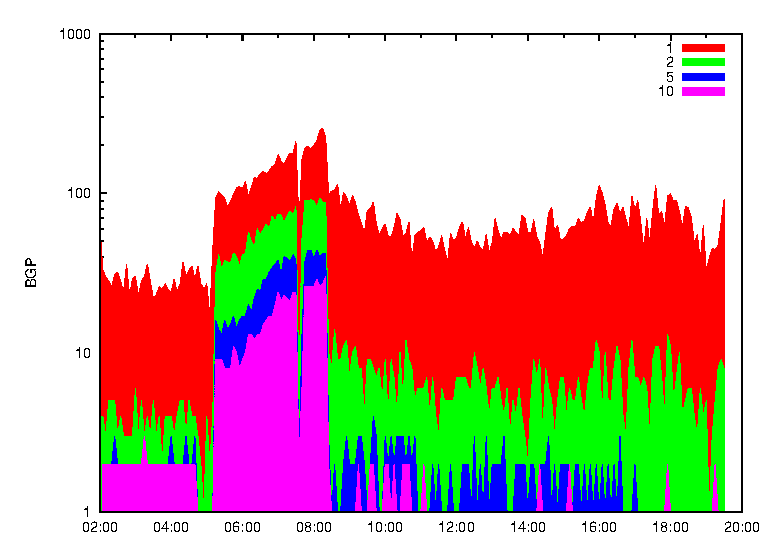
\includegraphics[width=0.75\linewidth]{images/events/2010_03_25/bgp_log_port80_ref.eps}
	\caption{Event 1: Unreachable BGP prefixes detected by the classical FACT traffic preselection based on the port-based heuristic.} 
	\label{fig:AMS_IX_FACT_REF} 
\end{figure}

\subsection{Server Socket Approach}
For evaluating the server socket bases approach, several different server socket sets are choosen, since this socket set selection process is an optimization problem as outlined in chapter \ref{chapter:integration}.

Firstly, a FACT is operated with a server socket set denoted as \emph{AllPort80SeS}, including all detected server socket listening on port 80. This socket set can directly be compared to the old heuristic approach, since it monitors a majority of those traffic as well. 

As figure \ref{fig:AMS_IX_FACT_allSES80} shows, the real event lasting from 05.00 UTC to 08:15 UTC is clearly visible equally well as in the heuristic approach from figure \ref{fig:AMS_IX_FACT_REF}. However, the server socket based approach reduces the red part indicating the number of unreachable prefixes affecting only a single internal user by at least an order of magnitude. Hence,  the event is now clearly standing out of the \emph{background event detection noise}.

Despite that fact, that the \emph{AllPort80SeS} set is not optimized at all, it outperformed the traditional approach in terms of noise reduction without significantly worsen the real event detection. This confirms the assumption that a high number of unreachable prefixes affecting only a single internal user is caused by malware and p2p churn.


\begin{figure}
	[p] \centering 
	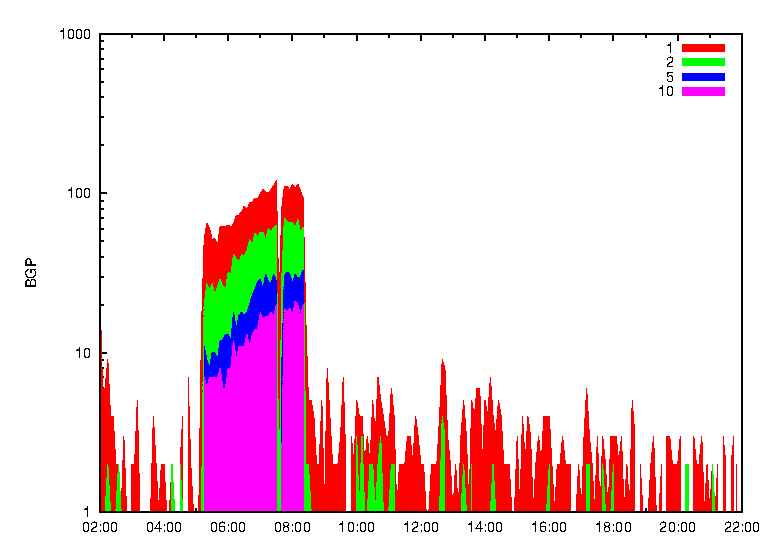
\includegraphics[width=0.75\linewidth]{images/events/2010_03_25/bgp_log_allPort80SES.eps}
	\caption{Event 1: Unreachable BGP prefixes detected by the modified FACT traffic preselection based on all port 80 server sockets.} 
	\label{fig:AMS_IX_FACT_allSES80} 
\end{figure}


\begin{figure}
	[p] \centering 
	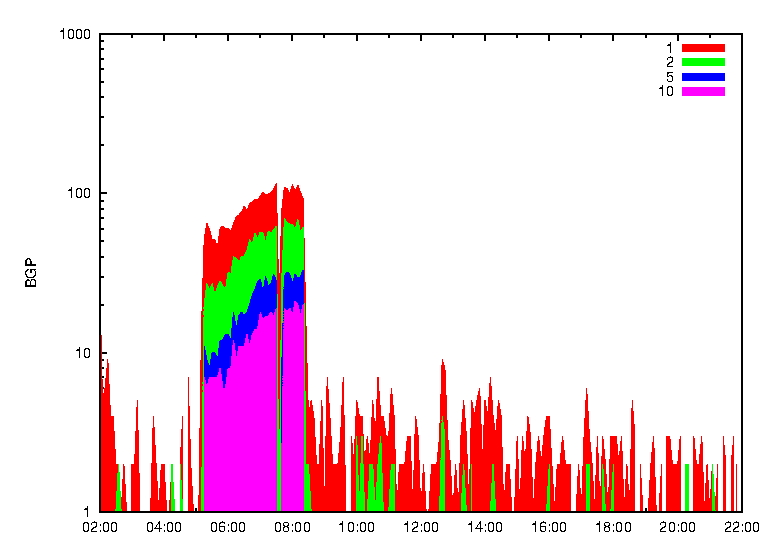
\includegraphics[width=0.75\linewidth]{images/events/2010_03_25/bgp_log_port80_Set_stab_0_vts_2.eps}
	\caption{Event 1: Unreachable BGP prefixes detected by the modified FACT traffic preselection based on all port 80 server sockets with visibility of at least 2 days.} 
	\label{fig:AMS_IX_FACT_allSES80VTS2} 
\end{figure}

\begin{figure}
	[p] \centering 
	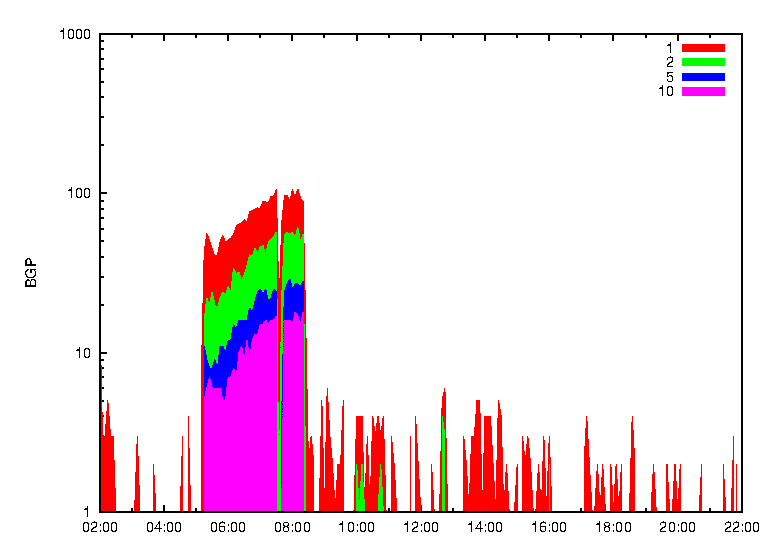
\includegraphics[width=0.75\linewidth]{images/events/2010_03_25/bgp_log_port80_Set_stab_9_vts_2.eps}
	\caption{Event 1: Unreachable BGP prefixes detected by the modified FACT traffic preselection based on all port 80 server sockets with visibility of at least 2 days and stability ratio of at least $90\%$.} 
	\label{fig:AMS_IX_FACT_allSES80VTS2STAB9} 
\end{figure}

\begin{figure}
	[p] \centering 
	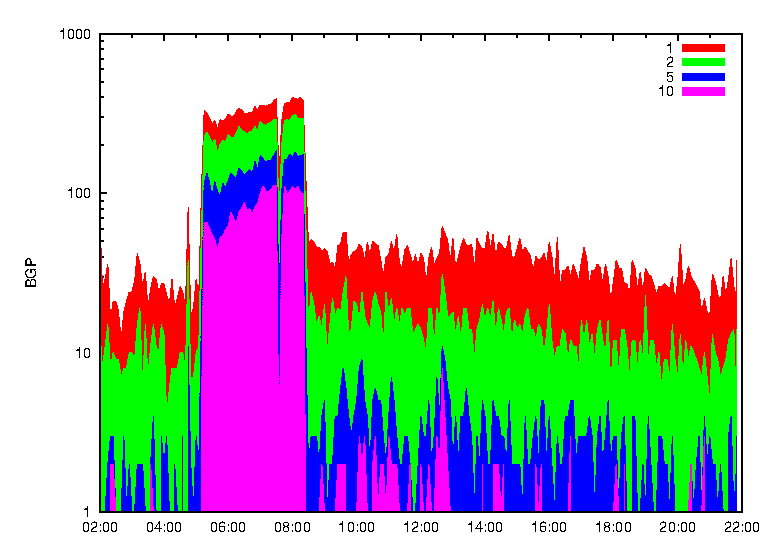
\includegraphics[width=0.75\linewidth]{images/events/2010_03_25/bgp_log_all_external.eps}
	\caption{Event 1: Unreachable BGP prefixes detected by the modified FACT traffic preselection based on all detected server sockets} 
	\label{fig:AMS_IX_FACT_allSES} 
\end{figure}

\begin{figure}
	[p] \centering 
	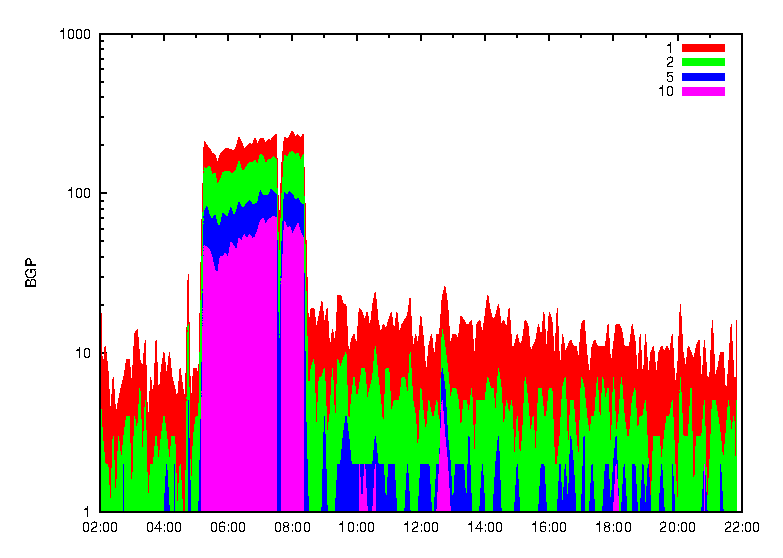
\includegraphics[width=0.75\linewidth]{images/events/2010_03_25/bgp_log_Set_var_0_1_stab_9_vts_2.eps}
	\caption{Event 1: Unreachable BGP prefixes detected by the modified FACT traffic preselection based on the $70\%$ most popular server sockets limited to those with a visibility of at least 2 days and stability ratio of at least $90\%$.} 
	\label{fig:AMS_IX_FACT_popularVTS2STAB9} 
\end{figure}


%%%%%%%%%%%%%%%%%%%%%%%%%%%%%%%%%%%%%%%%%%%%%%%%%%%%%%%%%%%%%%%%%%%%%%%%%%%%%%%%
% EVENT 2: TIER-1 BLACK-HOLING
%%%%%%%%%%%%%%%%%%%%%%%%%%%%%%%%%%%%%%%%%%%%%%%%%%%%%%%%%%%%%%%%%%%%%%%%%%%%%%%%
\newpage
\section{Event 2: Reverse Path Traffic Black-holing}

On May 18, 2010, the operators of the SWITCH network were assigned to investigate an reported issue that all services in an external /24 network were not accessible from the SWITCH network between 08:30 and 08:45 UTC. According to SWITCH, the problem was most likely due to an issue of an tier-1 provider which black-holed parts of the reverse traffic towards the SWITCH network\citep{SchatzmannPAM2011}.

Unfortunately, the operators were neither able to tell how many internal users were affected nor how many external networks were unreachable during this period of time. However with the help of FACT, this issue can be further assessed with respect to the severity of the event\citep{SchatzmannPAM2011}.

\subsection{Heuristic Approach}

\begin{figure}
	[p] \centering 
	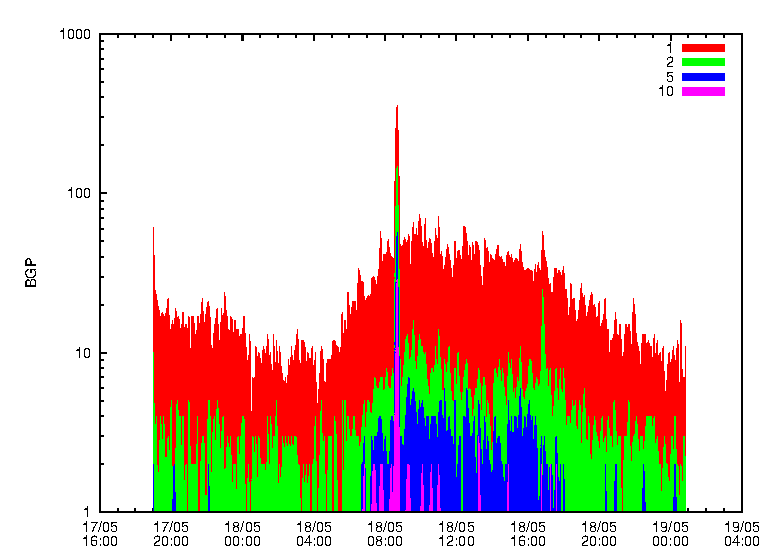
\includegraphics[width=0.75\linewidth]{images/events/2010_05_18/bgp_log_port80_ref.eps}
	\caption{Event 2: Unreachable BGP prefixes detected by the classical FACT traffic preselection based on the port-based heuristic.} 
	\label{fig:TIER1_FACT_REF} 
\end{figure}

\subsection{Server Socket Approach}

\begin{figure}
	[p] \centering 
	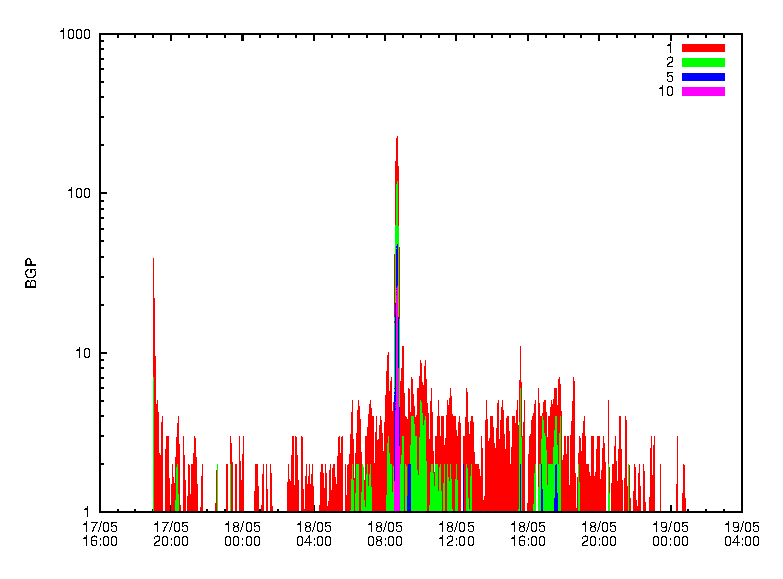
\includegraphics[width=0.75\linewidth]{images/events/2010_05_18/bgp_log_allPort80SES.eps}
	\caption{Event 2: Unreachable BGP prefixes detected by the modified FACT traffic preselection based on all port 80 server sockets.} 
	\label{fig:TIER1_FACT_allSES80} 
\end{figure}


\begin{figure}
	[p] \centering 
	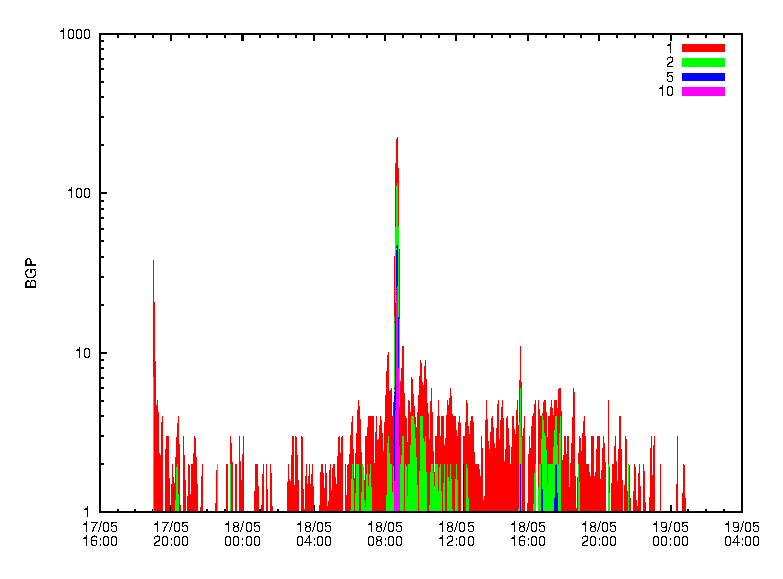
\includegraphics[width=0.75\linewidth]{images/events/2010_05_18/bgp_log_port80_Set_stab_0_vts_2.eps}
	\caption{Event 2: Unreachable BGP prefixes detected by the modified FACT traffic preselection based on all port 80 server sockets with visibility of at least 2 days.} 
	\label{fig:TIER1_FACT_allSES80VTS2} 
\end{figure}

\begin{figure}
	[p] \centering 
	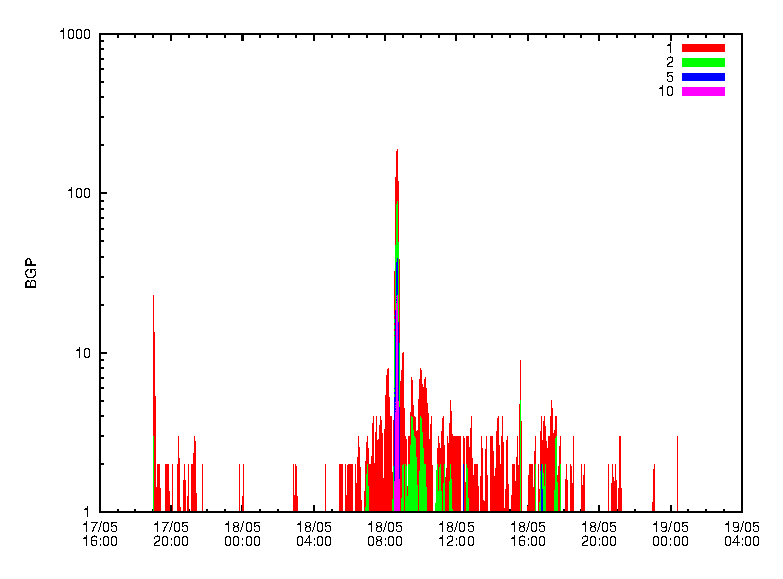
\includegraphics[width=0.75\linewidth]{images/events/2010_05_18/bgp_log_port80_Set_stab_9_vts_2.eps}
	\caption{Event 2: Unreachable BGP prefixes detected by the modified FACT traffic preselection based on all port 80 server sockets with visibility of at least 2 days and stability ratio of at least $90\%$.} 
	\label{fig:TIER1_FACT_allSES80VTS2STAB9} 
\end{figure}

\begin{figure}
	[p] \centering 
	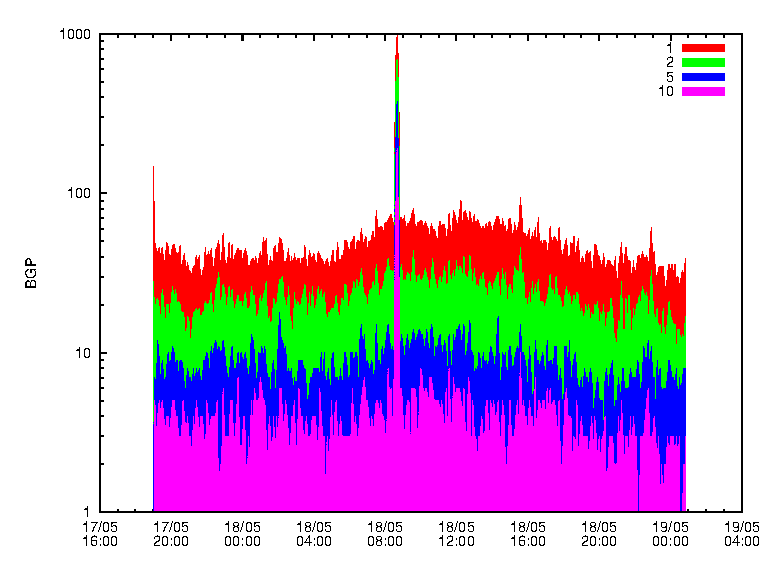
\includegraphics[width=0.75\linewidth]{images/events/2010_05_18/bgp_log_all_external.eps}
	\caption{Event 2: Unreachable BGP prefixes detected by the modified FACT traffic preselection based on all detected server sockets} 
	\label{fig:TIER1_FACT_allSES} 
\end{figure}


\begin{figure}
	[p] \centering 
	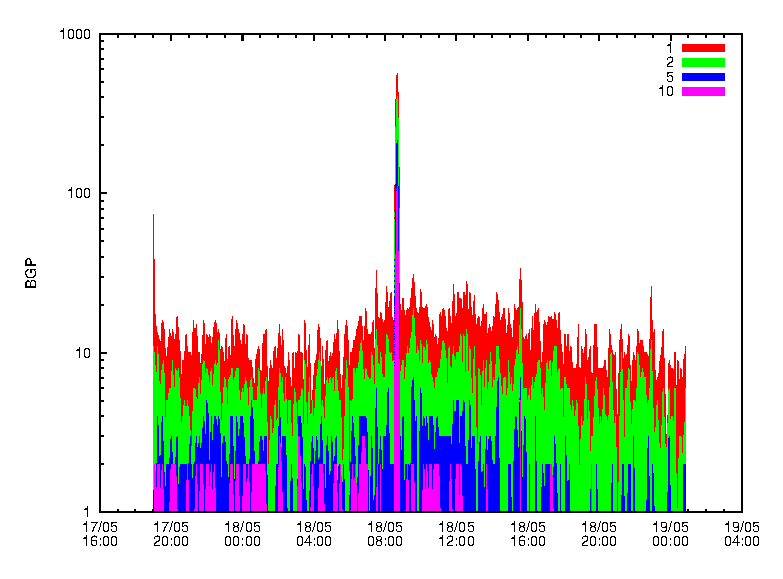
\includegraphics[width=0.75\linewidth]{images/events/2010_05_18/bgp_log_Set_var_0_1_stab_9_vts_2.eps}
	\caption{Event 2: Unreachable BGP prefixes detected by the modified FACT traffic preselection based on the $70\%$ most popular server sockets limited to those with a visibility of at least 2 days and stability ratio of at least $90\%$.} 
	\label{fig:TIER1_FACT_popularVTS2STAB9} 
\end{figure}

%%%%%%%%%%%%%%%%%%%%%%%%%%%%%%%%%%%%%%%%%%%%%%%%%%%%%%%%%%%%%%%%%%%%%%%%%%%%%%%%
% EVENT 3: RIPE / DUKE BGP EXPERIMENT
%%%%%%%%%%%%%%%%%%%%%%%%%%%%%%%%%%%%%%%%%%%%%%%%%%%%%%%%%%%%%%%%%%%%%%%%%%%%%%%%
\newpage
\section{Event 3: RIPE / DUKE BGP Experiments}

An experiment with new BGP attributes jointly performed by RIPE and the Duke 
University on August 27, 2010, resulted in several unreachable prefixes\citep{SchatzmannPAM2011}. These 
new kind of attributes has never been announced on the Internet before,  
although it was in accordance with the BGP specification\citep{ripe_duke}.

These new kind of attributes uncovered and triggered a bug in some Cisco BGP 
Routers known as the \emph{Cisco IOS XR Software Border Gateway Protocol Vulnerability (SA-20100827-BGP)}\citep{cisco_vulnerability}. In particular, the announcements with the new attributes were corrupted 
by the Cisco Routers and send to their peers. Consequently, their peers detected 
the corruption and dropped the entire peering session\citep{ripe_duke}.

\subsection{Heuristic Approach}

\begin{figure}
	[p] \centering 
	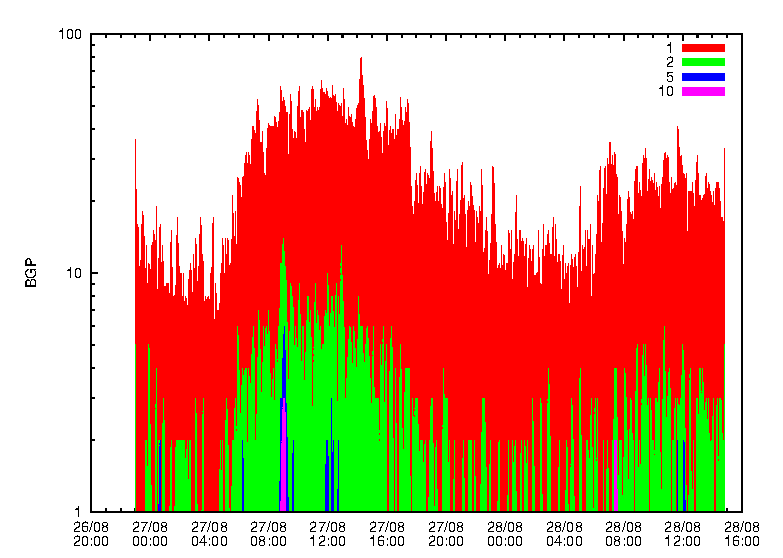
\includegraphics[width=0.75\linewidth]{images/events/2010_08_27/bgp_log_port80_ref.eps}
	\caption{Event 3: Unreachable BGP prefixes detected by the classical FACT traffic preselection based on the port-based heuristic.} 
	\label{fig:RIPE_FACT_REF} 
\end{figure}

\subsection{Server Socket Approach}

\begin{figure}
	[p] \centering 
	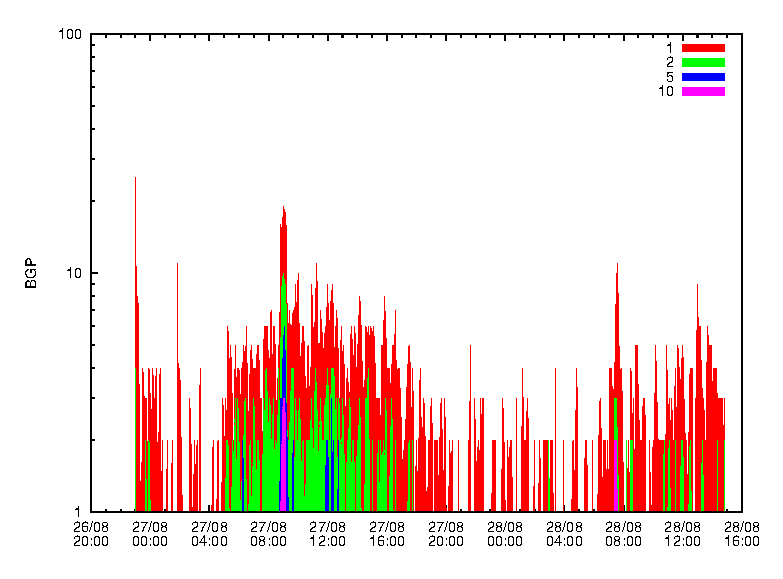
\includegraphics[width=0.75\linewidth]{images/events/2010_08_27/bgp_log_allPort80SES.eps}
	\caption{Event 3: Unreachable BGP prefixes detected by the modified FACT traffic preselection based on all port 80 server sockets.} 
	\label{fig:RIPE_FACT_allSES80} 
\end{figure}


\begin{figure}
	[p] \centering 
	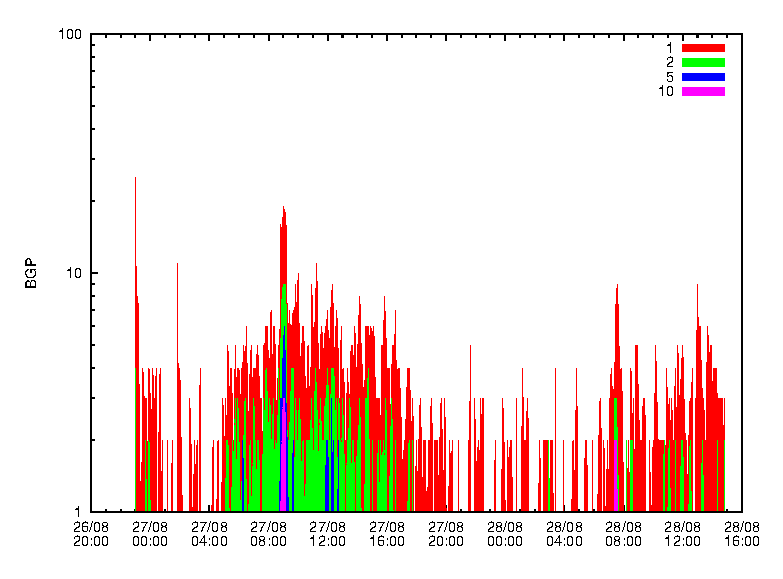
\includegraphics[width=0.75\linewidth]{images/events/2010_08_27/bgp_log_port80_Set_stab_0_vts_2.eps}
	\caption{Event 3: Unreachable BGP prefixes detected by the modified FACT traffic preselection based on all port 80 server sockets with visibility of at least 2 days.} 
	\label{fig:RIPE_FACT_allSES80VTS2} 
\end{figure}

\begin{figure}
	[p] \centering 
	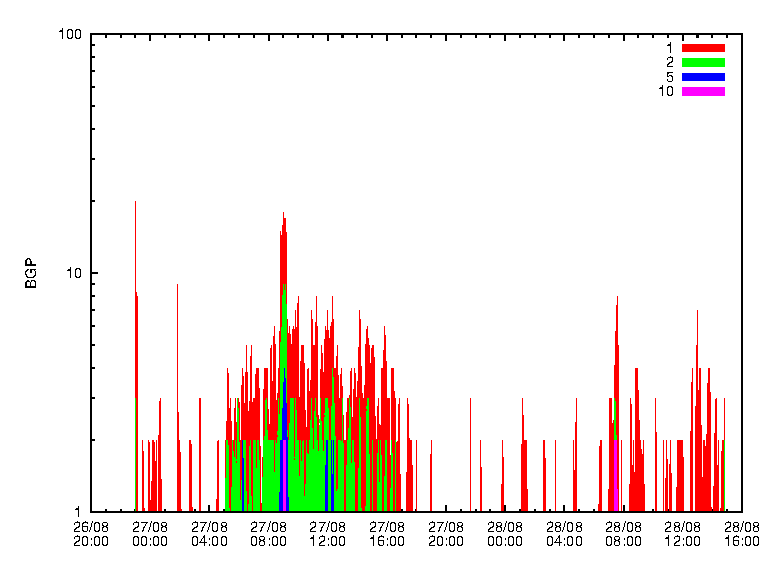
\includegraphics[width=0.75\linewidth]{images/events/2010_08_27/bgp_log_port80_Set_stab_9_vts_2.eps}
	\caption{Event 3: Unreachable BGP prefixes detected by the modified FACT traffic preselection based on all port 80 server sockets with visibility of at least 2 days and stability ratio of at least $90\%$.} 
	\label{fig:RIPE_FACT_allSES80VTS2STAB9} 
\end{figure}

\begin{figure}
	[p] \centering 
	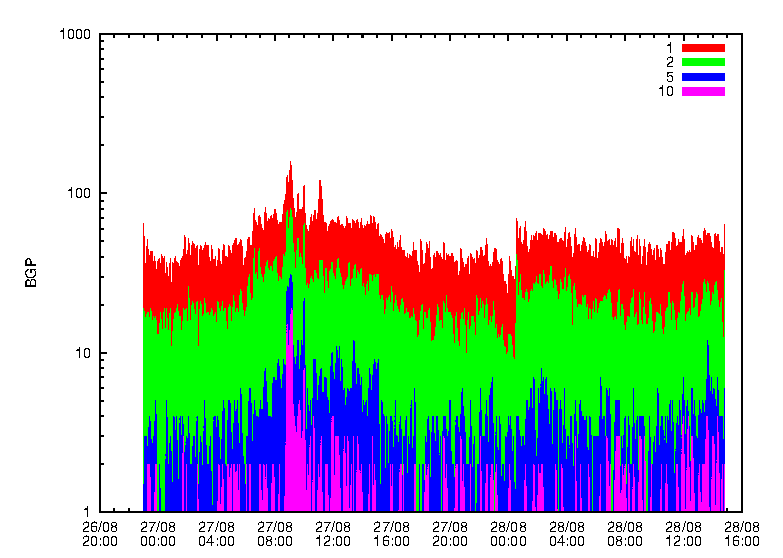
\includegraphics[width=0.75\linewidth]{images/events/2010_08_27/bgp_log_all_external.eps}
	\caption{Event 3: Unreachable BGP prefixes detected by the modified FACT traffic preselection based on all detected server sockets} 
	\label{fig:RIPE_FACT_allSES} 
\end{figure}

\begin{figure}
	[p] \centering 
	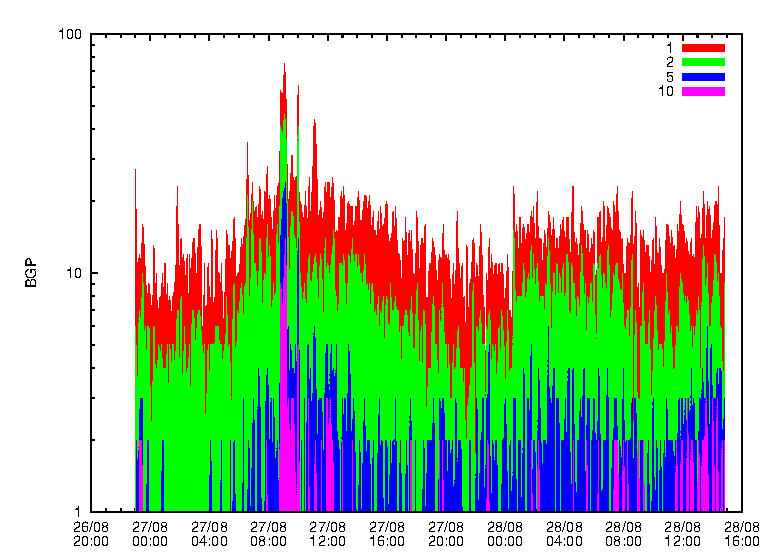
\includegraphics[width=0.75\linewidth]{images/events/2010_08_27/bgp_log_Set_var_0_1_stab_9_vts_2.eps}
	\caption{Event 3: Unreachable BGP prefixes detected by the modified FACT traffic preselection based on the $70\%$ most popular server sockets limited to those with a visibility of at least 2 days and stability ratio of at least $90\%$.} 
	\label{fig:RIPE_FACT_popularVTS2STAB9} 
\end{figure}

%%%%%%%%%%%%%%%%%%%%%%%%%%%%%%%%%%%%%%%%%%%%%%%%%%%%%%%%%%%%%%%%%%%%%%%%%%%%%%%%
% RESULTS
%%%%%%%%%%%%%%%%%%%%%%%%%%%%%%%%%%%%%%%%%%%%%%%%%%%%%%%%%%%%%%%%%%%%%%%%%%%%%%%%
\newpage
\section{Results}

